\subsection{Candidate gradient magnitudes}\label{app:gradient-norms}

\Cref{fig:gradient-norms} adds a step-level diagnostic before admission;
retained learning remains a separate question.

\begin{figure}[!tb]
  \setlength{\abovecaptionskip}{4pt}
  \centering
  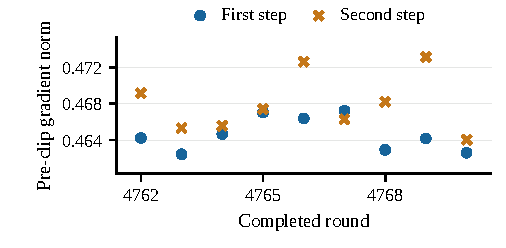
\includegraphics[width=\linewidth]{figures/fig_gradient_norms.pdf}
  \caption{\textbf{Candidate gradient norms vary across recorded steps.}
  All 9 complete retained summaries, rounds 4762--4770, captured at
  02:55 UTC on 4 November 2026. The 18 markers are logged pre-clip adapter
  gradient norms, two per candidate round. The steps use distinct training
  batches; their difference is not a matched loss reduction. No smoothing
  or filtering is applied. The window records zero admissions; these
  magnitudes establish no retained learning gain. Scope: \cref{sec:method-status}.}
  \label{fig:gradient-norms}
\end{figure}
